Process mining \cite{pm} is an ever-growing research field that provides a number of methods and algorithms aiming to help analyze and gain insight over processes.
Processes consist of sets of activities that are performed over some time span indicating the steps that were executed to complete a specific task or goal.
An ever-increasing number of businesses use \textit{Process-Aware Information Systems (PAISs)} as software tools to aid them in generating and managing digital records for every process-related step that is performed.
This information can then be extracted in the form of an \textit{event log}, a database that contains a number of unique events that were executed as part of particular runs of the process.
An event might be enclosed with information indicating the specific activity and the resource that performed it, the time it was executed, and other additional attributes.

The main entity in the process-view of the provided event data are the \textit{process instances}.
Each process instance is identified through a unique \textit{case ID}, an event attribute that assigns each event to a unique process run.
For this reason, we often use the terms case and process instance interchangeably.
Each case has a corresponding set of events that were executed in some order and during which particular activities were performed.
The \textit{activity} attribute enables obtaining the activity that was performed from each event from the event set belonging to any process instance, whereas the \textit{timestamp} attribute enables ordering the performed activities into a chronological sequence, called \textit{trace}.
The case ID, activity and timestamp are the three necessary event attributes that provide the \textit{control-flow} perspective of any process.
While each process instance has a corresponding timely ordered sequence of events, it is the projection of these events onto the corresponding executed activities, the \textit{traces}, which yield meaningful information.
Assuming that the data was recorded correctly, the traces are real examples of process runs, possibly containing many reoccurring patterns.
The more data are available, the higher the number of real examples from which one can conclude what the ``real'' process looks like.
Using data-driven algorithms that transform given multisets of traces into graphs and models that are as understandable, accurate and precise as possible is the main goal of \textit{process discovery}.
Discovery algorithms typically produce models in the form constructs such as Petri Nets, BPMN models, and Process Trees.
Many commercial tools, however, produce models in the form of  \textit{Directly-Follows-Graphs (DFGs)}.
In DFGs, nodes stand for recorded activities, whereas directed arcs connect activity pairs whenever they were recorded happening consecutively.
Another important task in process mining is \textit{conformance checking}, whose aim is to compare recorded with expected or prescribed process behavior.
A challenge in conformance checking is discovering methods that are both efficient and robust in measuring at what degree the recorded process runs conform to the allowed behavior indicated by a prescriptive model.
Process mining methods provide insight and diagnostics derived from real event data.
Taking active decisions to change the process based on that knowledge may lead to overall improved processes which may be more efficient, have lower risks, ensure greater customer satisfaction, reduce bottlenecks, and prevent fraud.\\
The quality of the insights that process mining methods provide depends, however, on the quality of the recorded data.
The data may be noisy, containing spurious, inconsistent or missing values.
If the inaccurate or noisy values are infrequent, this problem is usually addressed by removing the affected records from the data that will be later used for analysis.
If on the other hand, the inaccuracies are frequent and pervasive, filtering methods may cause too much information loss and make the data unusable.
In our work, we assume that event data is \textit{uncertain}, in the sense that the event attributes do not always contain unique values.
This uncertainty is \textit{explicit}, since events are enclosed with a formal description of the possible values of the affected attributes.
The framework we use for classifying and handling event data with explicit uncertainty was first introduced in \cite{mining}.
We distinguish two types of uncertainty:
\begin{itemize}
\item \textit{Strong uncertainty}: a set or a range of possible attribute values is known, but the information regarding their distribution is missing or is unobtainable. 
\item \textit{Weak uncertainty}: both the possible values and their corresponding distribution are at disposal.
\end{itemize}
%
%
%
%
%
\begin{figure}[htp]
  \centering
 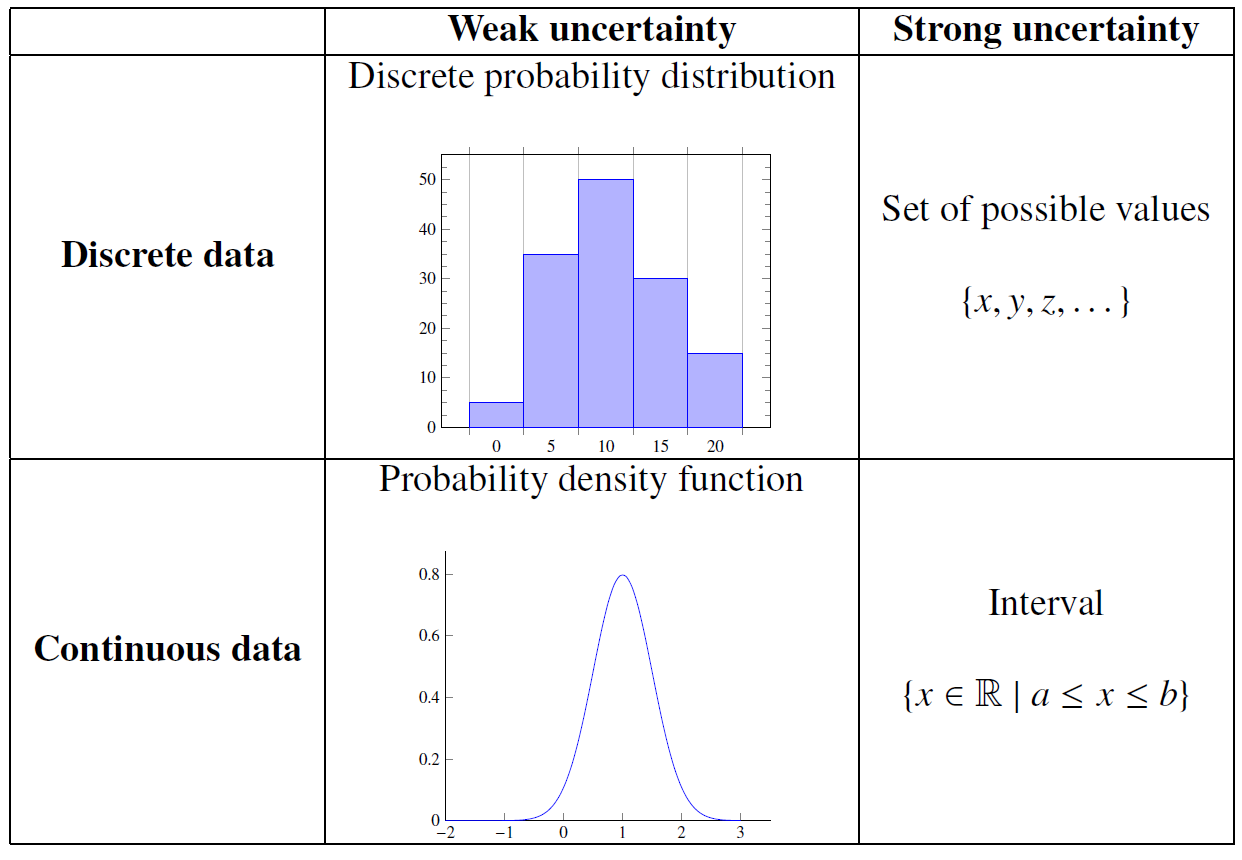
\includegraphics[width=12cm]{figures/unctypes.png}
	\caption{The four different types of uncertainty \cite{conformance}.}
	\label{fig: uncertainty types}
\end{figure}
%
%
%
%
%
Fig. \ref{fig: uncertainty types} from \cite{conformance} summarizes these types of uncertainty both for discrete and continuous domains.
There are various reasons which might cause uncertainty in the recorded event data.
Recordings might be prone to human errors if the data is inserted manually.
On the other hand, software errors might affect the data in unpredictable ways.
Under such circumstances, the data may display many quality issues including incorrectness, ambiguity, inconsistency, coarseness and so on.
Such factors, however, only \textit{imply} uncertainty in the data.
Describing uncertainty explicitly may be done straightforwardly or with the help of a domain expert.
If the recorded timestamps are too coarse, e.g. only the date but not the exact time is recorded, then the uncertain timestamps correspond to a time interval whose extremes are the start and end of the corresponding day.
If the executed activity of a particular event is not recorded, then knowing the resource who executed that event might indicate that the possible activities correspond to the tasks usually performed by that resource.
The uncertainty accompanying recorded measurements might also be explicit beforehand.
For instance, sensors might have an error model that follows a normal distribution around the measured value.
In this work, we focus on the uncertainty affecting two of the control-flow attributes: activity and timestamp.
Additionally, we account for events whose execution is uncertain, which we call \textit{indeterminate} events.
As explained in \cite{mining}, imprecise recordings are not removed from the data, either because it would make the data useless, or becuase the imprecision is known, expected or unavoidable.
Instead, uncertainty is explicitly modeled in graph-type structures \citep{mining,discovery,conformance}, which enable the application of existing discovery and conformance checking methods to uncertain data.
%
%
%
%
\begin{table}[htp]
\caption{An example showing the recorded events of some uncertain process instance.}
	\centering
	\begin{tabular}{ccccc}
		\textbf{Case ID} & \textbf{Event ID}        & \textbf{Activity}                                                                                                     & \textbf{Timestamp}             & \multicolumn{1}{l}{\textbf{Event Type}} \\ \hline
		\multicolumn{1}{|c|}{3716} & \multicolumn{1}{|c|}{$e_1$} &
		\multicolumn{1}{c|}{$a$} & \multicolumn{1}{c|}{\begin{tabular}[c]{@{}c@{}} 10:00\end{tabular}}                                                                                 & \multicolumn{1}{c|}{!}                    \\ \hline
		\multicolumn{1}{|c|}{3716} & \multicolumn{1}{|c|}{$e_2$} &
		\multicolumn{1}{c|}{$\{b,c\}$} & \multicolumn{1}{c|}{\begin{tabular}[c]{@{}c@{}}[12:00, 13:30]\end{tabular}}                                                                         &  \multicolumn{1}{c|}{!}                    \\ \hline
		\multicolumn{1}{|c|}{3716} & \multicolumn{1}{|c|}{$e_3$} &
		\multicolumn{1}{c|}{$d$}        & \multicolumn{1}{c|}{\begin{tabular}[c]{@{}c@{}}[12:30, 14:00]\end{tabular}}                                                                          &	\multicolumn{1}{c|}{?}                    \\ \hline
		\multicolumn{1}{|c|}{3716} & \multicolumn{1}{|c|}{$e_4$} &
		\multicolumn{1}{c|}{$\{c:0.8,e:0.2\}$} & \multicolumn{1}{c|}{\begin{tabular}[c]{@{}c@{}}15:00\end{tabular}}                                                                         &  \multicolumn{1}{c|}{!}                    \\ \hline
		\multicolumn{1}{|c|}{3716} & \multicolumn{1}{|c|}{$e_5$} &
		\multicolumn{1}{c|}{$e$} & \multicolumn{1}{c|}{\begin{tabular}[c]{@{}c@{}}[14:30, 15:30]\end{tabular}}                                                                         &  \multicolumn{1}{c|}{!}                    \\ \hline
		\end{tabular}
		\label{table: table1}
\end{table}
%
%
%
%

Table \ref{table: table1} shows the recorded events of some uncertain process instance identified through case ID 3716.
During event $e_2$, one of the activities $b$ or $c$ were executed some time between 12:00 and 13:30.
The timestamps of events $e_3$ and $e_5$ are also given as an interval, while event $e_3$ is indeterminate.
During event $e_4$, either $c$ or $e$ were performed with a probability of $0.8$ and $0.2$ respectively.

Process instances with uncertain events present a number of challenges.
Most process mining techniques revolve around traces, and each case is assumed to have a unique corresponding trace of activities.
In the uncertain scenario, however, a single case might have many possible traces, which we often refer to as \textit{trace realizations}.
In the example case from Table \ref{table: table1}, sequences $\langle a,b,d,c,e\rangle$, $\langle a,d,c,c,e\rangle$ and $\langle a,b,d,e,e\rangle$ are some of the possible traces.
Because of uncertainty in activities, a single event sequence might execute more than one activity sequence.
For example, the event sequence $\langle e_1,e_2,e_3,e_4,e_5 \rangle$ belonging to the case from Table \ref{table: table1} might execute 4 distinct traces: $\langle a,b,d,c,e \rangle$, $\langle a,c,d,c,e \rangle$, $\langle a,b,d,e,e \rangle$, and $\langle a,c,d,e,e\rangle$.
Indeterminate events on the other hand also affect the set of activities performed during the process execution.
Trace $\langle a,b,c,e \rangle$ is a possible trace for the case in the example which does not contain activity $d$.
The most critical source of uncertainty are timestamps.
When events of a single case have possible time intervals which are overlapping, then a total order between those events is not obtainable any more.
Instead, the events are only \textit{partially ordered}, leading to all permutations of that event set being candidates for a possible event ordering.
In the example process instance from Table \ref{table: table1}, event $e_2$ overlaps with event $e_3$, and event $e_4$ overlaps with event $e_5$.
In our work, we introduce an algorithm to compute the set of possible event orderings.
Our method proves to be more efficient than the baseline method of checking all permutations when the input event set can be partitioned into smaller comparable subsets.
Moreover, we provide formulas for obtaining a probability estimate for every possible trace of an uncertain case depending on the uncertainty type, which is additionally defined on the case level.
We assume that the uncertainty information given on any event attribute is independent both from the other attributes of the same event, and from the attributes of other recorded events.
We also distinguish traces of events from traces of activities, and show which event attributes affect the likelihood of event orderings and which ones affect the likelihood of executing a particular activity sequence.
We use conformance checking as a motivating example on incorporating the probability estimates.
Similar to \cite{por}, we assign each uncertain process instance a conformance cost which is obtained by weighing the individual conformance scores of each possible trace by their corresponding probabilities.
Furthermore, we show how to obtain additional probability estimates for the trace realizations based on the behavioral regularities of the log by adapting the methods proposed in \cite{por} to fit our broader definition of uncertainty.

The remainder of this work is organised the following way: Chapter \ref{chap:related_work} gives an overview of related work concerning uncertain event data and partial orders.
Chapter \ref{chap:prelim} contains the basic definitions needed to model and classify uncertain data, while Chapter \ref{chap:fundamentals} introduces important concepts for handling uncertain process instances based on previous work from Pegoraro et al. \citep{mining,discovery,efficient,conformance}.
In Chapter \ref{chap:realizations}, we introduce an algorithm for computing the possible event traces of an uncertain case, and we analyze its runtime both theoretically and experimentally.
In Chapter \ref{chap:estimates}, we propose methods to compute a probability distribution over the trace realizations of a particular process instance, using the uncertainty information enclosing its corresponding events.
Through small examples we demonstrate how the probabilities might affect conformance checking costs.
The estimated probabilities are validated in an example using a Monte Carlo Simulation approach.  
In Chapter \ref{chap:logpatterns}, we show how another probability distribution over the possible traces can be computed using inter-trace information in the form of behavioral regularities in the log.
Finally, \mbox{Chapter \ref{chap:conclusion}} concludes the thesis and discusses ideas for future work.




%
%
%
%
%
%
%
